%%%%%%%%%%%%%%%%%%%%%%%%%%%%%%%%%%%%%%%%%%%%%%%%%%%%%%%%%%%%%%%%%%%%%%
% Lớp 11 | Hàm số lượng giác và phương trình lượng giác | [Giảm] Phương trình lượng giác thường gặp
% Dạng 1D1?6-8: Toán thực tế áp dụng phương trình lượng giác thường gặp
% Số câu: 2  (sinh tự động bởi tach_cau.py; từ nay thầy sửa trực tiếp file này)
%%%%%%%%%%%%%%%%%%%%%%%%%%%%%%%%%%%%%%%%%%%%%%%%%%%%%%%%%%%%%%%%%%%%%%

%%%%%%%%%%%%%%%% TRẢ LỜI NGẮN %%%%%%%%%%%%%%%%

% nguồn: Ok_TraLoiNgan_Lop11_Lan1
\begin{ex}%[1D1N6-8]%[ma:67c0346d]
	Hằng ngày mực nước tại một cảng biển lên xuống theo thuỷ triều. Độ sâu $h$ m của mực nước theo thời gian $t$ (giờ) trong một ngày được cho bởi công thức 
	\centerline{$h=11+2\sin\left(\dfrac{\pi}{12}t\right) ~\text{với}  ~0\leq t\leq 24$.}
	Tìm thời điểm mà mực nước tại cảng là  cao nhất.
	 \shortans{6}
	 \loigiai{
		Ta có 
		\begin{eqnarray*}
			&&-1\le\sin\left(\dfrac{\pi}{12}t\right)\le 1\\ 
			&\Leftrightarrow & 11-2\le  11+2\sin\left(\dfrac{\pi}{12}t\right)\le 11+2\\
			&\Leftrightarrow& 9\le h\le  13
		\end{eqnarray*}
		Vậy mực nước tại cảng cao nhất bằng  $13$ m khi
		\begin{eqnarray*}
			 &&\sin\left(\dfrac{\pi}{12}t\right)=1\\
			&\Leftrightarrow &  \left(\dfrac{\pi}{12}t\right)=\dfrac{\pi}{2}+2k\pi\\
			&\Leftrightarrow & t=6+24k  ~\left(k\in\mathbb{Z}\right).
		\end{eqnarray*}
		Mà $0\le t\le 24$ nên $t=6$.\\ Vậy thời điểm mà mực nước tại cảng cao  nhất là lúc $6$ (giờ).
	} 
\end{ex}

% nguồn: Ok_TraLoiNgan_Lop11_Lan1
\begin{ex}%[1D1V6-8]%[ma:42b6b9f7]
	Trong hình dưới, khi được kéo ra khỏi vị trí cân bằng ở điểm $O$ và buông tay, lực đàn hồi của lò xo khiến vật $A$ gắn ở đầu của lò  xo dao động quanh $O$. Toạ độ $s$ (cm) của $A$ trên trục $Ox$ vào thời điểm $t$ (giây) sau khi buông tay được xác định bởi công thức $s=10 \sin \left(10 t+\dfrac{\pi}{2}\right)$. Trong $10$ giây đầu tiên thì vật đi qua vị trí $s=-5 \sqrt{3}$ cm bao nhiêu lần?
	\begin{flushright}
		 \textit{(Theo https://www.britannica.com/science/simple-harmonic-motion)}
	\end{flushright}
	\begin{center}
		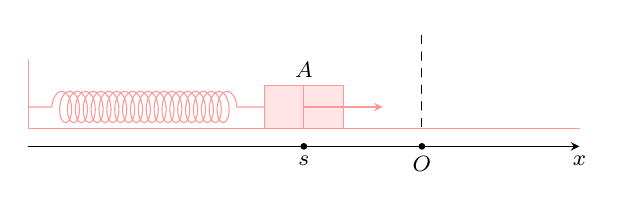
\begin{tikzpicture}[scale=1,font=\footnotesize,line join=round,line cap=round,>=stealth]
				\draw[red!40] (0,.6)--(0,-.27)--(7,-.27); 
				\draw[red!40,fill=red!10]  (3,-0.27) rectangle (3.5,.27)
					(3.5,-0.27) rectangle  (4,.27);
				\draw[red!40,->] (3.5,0)--(4.5,0); 
				\draw[red!40] 
					[ 
					 decoration={
					 coil,
					segment length  = 1mm,
					amplitude =  2mm,
					aspect  = 0.5,
					 post length = 3mm,
					pre length =  3mm},
					 decorate] (0,0) -- ++(3,0);
				 \draw[,->] (0,-.5) -- (7,-.5) node[below] {$x$};
				\draw[fill=black] 
					(3.5,-.5) circle (1pt) node[below]  {$s$}
					 (5,-.5) circle (1pt) node[below] {$O$}
					(3.5,.25) node[above]  {$A$};
				 \draw[dashed] (5,-0.25)--(5,1);
			\end{tikzpicture}
	\end{center}
	 \shortans{32}
	 \loigiai{
		 Theo giả thiết, ta có
		\allowdisplaybreaks 
		\begin{eqnarray*}
			&&10  \sin \left(10 t+\dfrac{\pi}{2}\right)=-5\sqrt{3}
			\Leftrightarrow \sin \left(10  t+\dfrac{\pi}{2}\right)=-\dfrac{\sqrt{3}}{2}\\
			 &\Leftrightarrow & \sin \left(10 t+\dfrac{\pi}{2}\right)=\sin\left(-\dfrac{\pi}{3}\right)
			\Leftrightarrow \hoac{&10t+\dfrac{\pi}{2}=-\dfrac{\pi}{3}+k2\pi \\&10  t+\dfrac{\pi}{2}=\pi+\dfrac{\pi}{3}+l2\pi \\} \\
			&\Leftrightarrow  &\hoac{&t=-\dfrac{\pi}{12}+\dfrac{k\pi}{5} \\&t=\dfrac{\pi}{12}+\dfrac{l\pi}{5} \\} (k, l\in \mathbb{Z}).
		\end{eqnarray*}
		Vậy để $s=-5\sqrt{3}$ cm thì $t=-\dfrac{\pi}{12}+\dfrac{k\pi}{5}$, $(k \in  \mathbb{N}^*)$ và $t=\dfrac{\pi}{12}+\dfrac{l\pi}{5}$, $(l\in \mathbb{N})$. \\
		Xét  $\hoac{&0\leq -\dfrac{\pi}{12}+\dfrac{k\pi}{5}\leq 10 \\
		&0\leq \dfrac{\pi}{12}+\dfrac{l\pi}{5}\leq  10}
		\Leftrightarrow \hoac{&\dfrac{5}{12}\leq k\leq \dfrac{50}{\pi}+\dfrac{5}{12} 
		 \rightarrow k\in \{1; 2; \ldots; 16\} \\
		&-\dfrac{5}{12}\leq l\leq \dfrac{50}{\pi}-\dfrac{5}{12}\rightarrow l\in \{0; 1; 2; \ldots; 15\}.}$\\ 
		Vậy trong  $10$ giây đầu tiên, vật đi qua vị trí $s=-5\sqrt{3}$ cm $32$ lần.
	 }
\end{ex}
